\documentclass[fontset=windows]{article}
\usepackage[margin=1in]{geometry}
\usepackage{ctex}
\usepackage{setspace}
\usepackage{lipsum}
\usepackage{graphicx}
\usepackage{caption}
\usepackage{subcaption}
\usepackage[colorlinks=true,linkcolor=red]{hyperref}
\usepackage{amsmath}
\usepackage{lmodern}

\graphicspath{{figures/}}

\title{\heiti\zihao{2} Nonlinear Op Amp Circuits \& Op Amp Nonidealities}
\author{\songti zrrraa}
\date{2023.12.23}

\begin{document}
\maketitle
\thispagestyle{empty}

\section*{Precision Rectifier}

\begin{figure}[htbp]
    \centering
    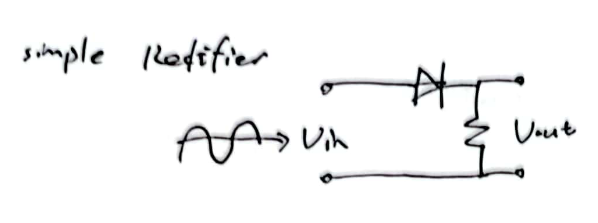
\includegraphics[scale=0.7]{1.jpg}
    \captionsetup{labelformat=empty}
    \caption{}
    \label{1}
\end{figure}

For general simple rectifiers, usually built by a diode, when the input voltage amplitude is very small, it can not reach the on-voltage of the diode, and it can not be rectified. 

\begin{figure}[htbp]
    \centering
    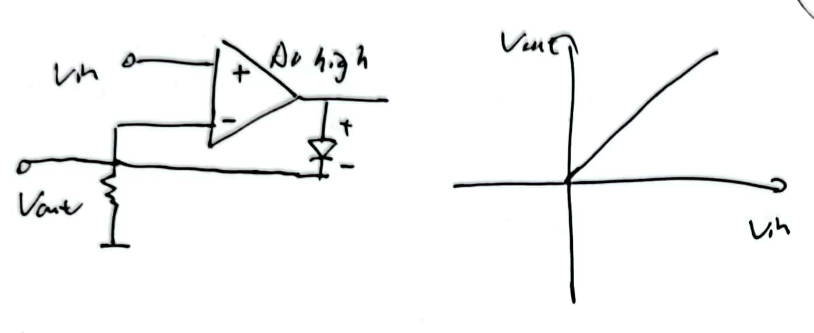
\includegraphics[scale=0.7]{2.jpg}
    \captionsetup{labelformat=empty}
    \caption{}
    \label{2}
\end{figure}

If constructed with an op amp, because $V_{in}\approx V_{out}$, no matter how small an input may be allowed to pass, multiply the difference between the op amp positive and negative inputs by the open loop gain equal to the on-voltage plus input. 

The relationship between input and output is shown below. 

When the input is negative, the op amp is saturated because the inverse input of the op amp cannot be negative. Operational release dead. 

\begin{figure}[htbp]
    \centering
    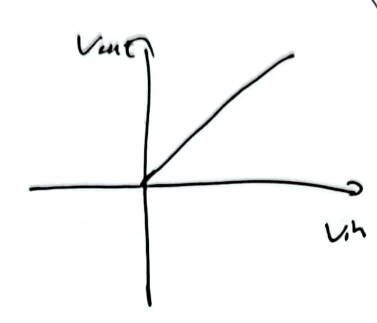
\includegraphics[scale=0.7]{3.jpg}
    \captionsetup{labelformat=empty}
    \caption{}
    \label{3}
\end{figure}

\section*{Logarithmic Amplifier}

\begin{figure}[htbp]
    \centering
    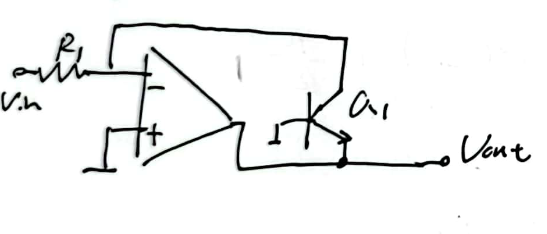
\includegraphics[scale=0.7]{4.jpg}
    \captionsetup{labelformat=empty}
    \caption{}
    \label{4}
\end{figure}

Using the logarithmic relationship between the collector current of the triode and the BE terminal voltage, we can build a logarithmic operational amplifier. 

$$\frac{V_{in}}{R_1}=I_{C1}=I_s*e^{\frac{V_{BE}}{V_T}}$$

$$V_{BE}=-V_{out}$$

$$V_{out}=-V_T*ln(\frac{V_{in}}{R_1I_s})$$

If $V_{in}<0$, Op Amp will saturate. The Op Amp is dead, is not defined. 

Similarly, we have another logarithmic op amp as follows. 

\begin{figure}[htbp]
    \centering
    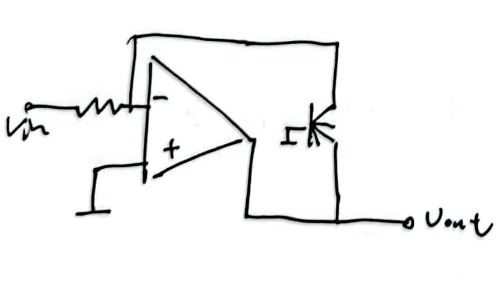
\includegraphics[scale=0.8]{5.jpg}
    \captionsetup{labelformat=empty}
    \caption{}
    \label{5}
\end{figure}

$$\frac{-V_{in}}{R_1}=I_s*e^{\frac{V_{EB}}{V_T}}$$

$$V_{out}=V_{EB}$$

$$V_{out}=V_T ln(\frac{V_{in}}{R_1I_s})$$

\section*{Imperfections of Op Amp}

\subsection*{DC Offsets}

\begin{figure}[htbp]
    \centering
    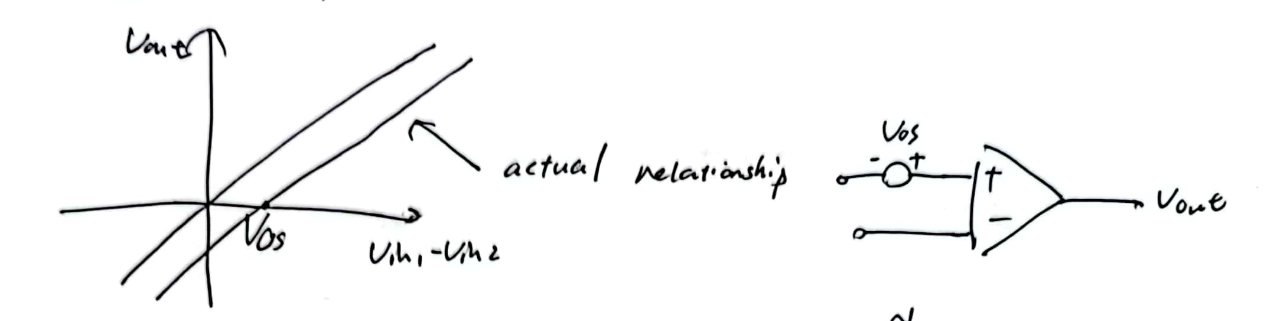
\includegraphics[scale=0.6]{6.jpg}
    \captionsetup{labelformat=empty}
    \caption{}
    \label{6}
\end{figure}

In fact, due to production process problems, the two inputs of the op amp may have random DC bias voltages. These random errors conform to the Gaussian distribution, generally between -2mV and +2mV. 

\begin{figure}[htbp]
    \centering
    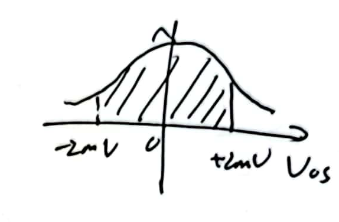
\includegraphics[scale=0.8]{7.jpg}
    \captionsetup{labelformat=empty}
    \caption{}
    \label{7}
\end{figure}

$V_{os}$ can be placed in series with either input. 

\subsection*{Effect of Offset on Amplifier}

\begin{figure}[htbp]
    \centering
    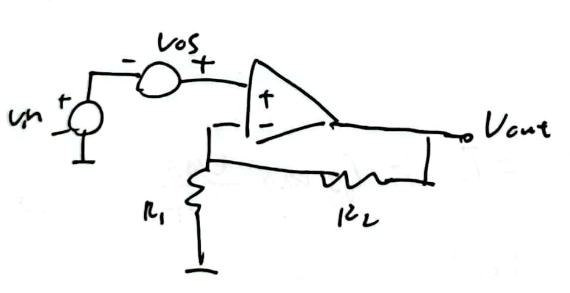
\includegraphics[scale=0.8]{8.jpg}
    \captionsetup{labelformat=empty}
    \caption{}
    \label{8}
\end{figure}

$$V_{out}=(V_{in}+V_{os})(1+\frac{R_2}{R_1})$$

\begin{figure}[htbp]
    \centering
    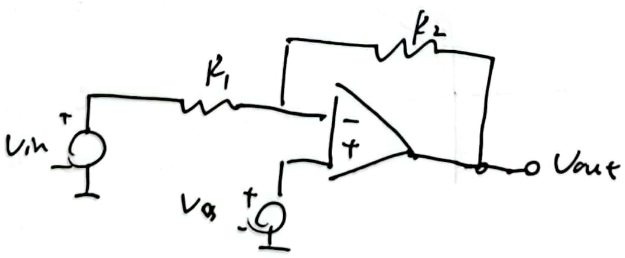
\includegraphics[scale=0.8]{9.jpg}
    \captionsetup{labelformat=empty}
    \caption{}
    \label{9}
\end{figure}

$$V_{out}=-\frac{R_2}{R_1}V_{in}+V_{os}(1+\frac{R_2}{R_1})$$

\subsection*{Effect of DC Offsets on Integrator}

\begin{figure}[htbp]
    \centering
    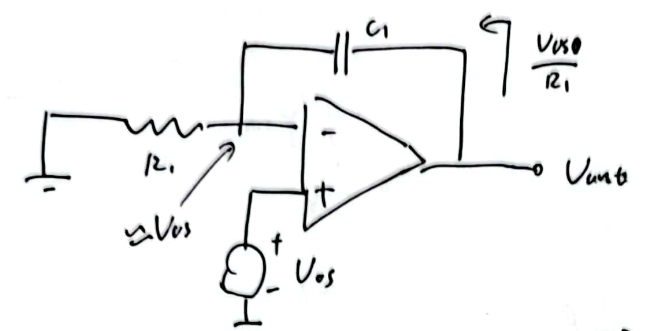
\includegraphics[scale=0.8]{10.jpg}
    \captionsetup{labelformat=empty}
    \caption{}
    \label{10}
\end{figure}

Due to $I=C\frac{dV}{dt}$

We can get: 

$$V=\frac{1}{C}\int Idt$$

$$V_{out}-V_{os}=\frac{1}{C_1}\int \frac{V_{os}}{R_1}dt$$

$$\Longrightarrow V_{out}=V_{os}+\frac{V_{os}}{C_1R_1}t$$

The circuit self-integrates its own DC bias. 

\begin{figure}[htbp]
    \centering
    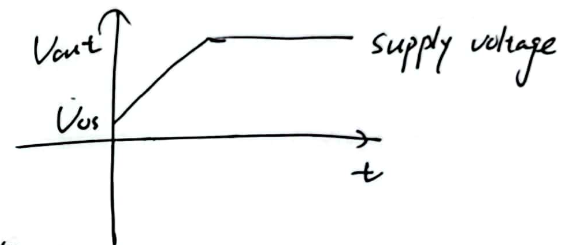
\includegraphics[scale=0.8]{12.jpg}
    \captionsetup{labelformat=empty}
    \caption{}
    \label{12}
\end{figure}

To fix the circuit: 

\begin{figure}[htbp]
    \centering
    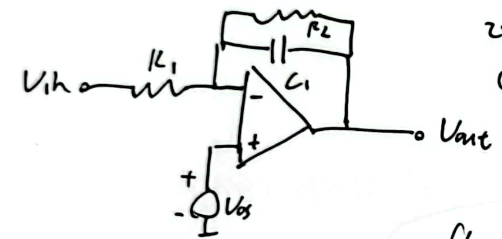
\includegraphics[scale=0.8]{11.jpg}
    \captionsetup{labelformat=empty}
    \caption{}
    \label{11}
\end{figure}

If $V_{in}=0$: 

$$V_{out}=(1+\frac{R_2}{R_1})V_{os}$$

$\frac{V_{os}}{R_1}$ prefers to flow throw resistor rather than capacitor at $t=\infty$. 

Ideal integrator transfer function is $-\frac{1}{R_1C_1s}$, our new integrator transfer function is: 

$$\frac{V_{out}}{V_{in}}\approx -\frac{\frac{R_2}{R_2C_1s+1}}{R_1}=-\frac{R_2}{R_1(R_2C_1s+1)}$$

To be a good integrator, the circuit requires that $|R_2C_1s|>>1$. 

In general, adding a resistor lets the DC bias flow through the resistor, preventing the DC bias from integrating itself. However, if the op amplifier wants to have a good integration effect on the AC signal, it requires that the DC and AC distinctions are obvious, that is, the input signal frequency should be large enough. 

In this way, the DC bias tends to flow through the resistor and the AC signal tends to flow through the capacitor. 

\subsection*{Input Bias Currents}

In the previous analysis, we consider that the input impedance of the op amp is infinite, and there is no current inflow at the positive and inverting inputs. In a real situation, there will be a current flowing in from the input. 

\begin{figure}[htbp]
    \centering
    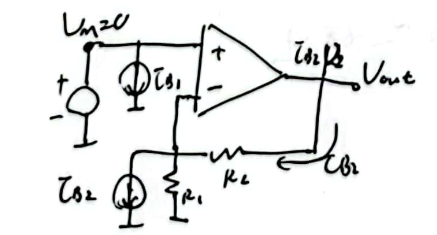
\includegraphics[scale=0.8]{13.jpg}
    \captionsetup{labelformat=empty}
    \caption{}
    \label{13}
\end{figure}

$I_{B1}$ and $I_{B2}$ are the input bias currents of the op amp. 

Consider that the input is 0, and the positive input has no current and no voltage. There is a loop at the inverting input, and the current flows from the output back to the input. 

The inverting input and the positive input have the same voltage of 0, so no current flows through $R_1$. 

Therefore, the current flowing through $R_2$ is $I_{B2}$. 

$$V_{out}=I_{B2}R_2$$

To fix the circuit: 

\begin{figure}[htbp]
    \centering
    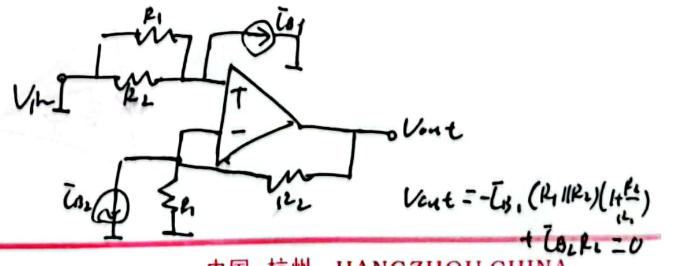
\includegraphics[scale=0.6]{14.jpg}
    \captionsetup{labelformat=empty}
    \caption{}
    \label{14}
\end{figure}

If we let: 

$$V_{out}=I_{V_{B1}}(R_1||R_2)(1+\frac{R_1}{R_2})+I_{B2}R_2=0$$

The DC bias current cancels out. 

\subsection*{Input Bias Currents in Integrator}

\begin{figure}[htbp]
    \centering
    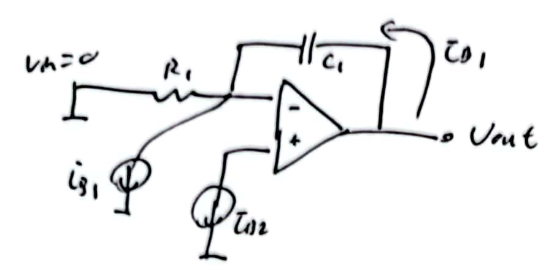
\includegraphics[scale=0.6]{15.jpg}
    \captionsetup{labelformat=empty}
    \caption{}
    \label{15}
\end{figure}

There is a self-integration of the DC bias current between the output and the input. 

To fix: 

\begin{figure}[htbp]
    \centering
    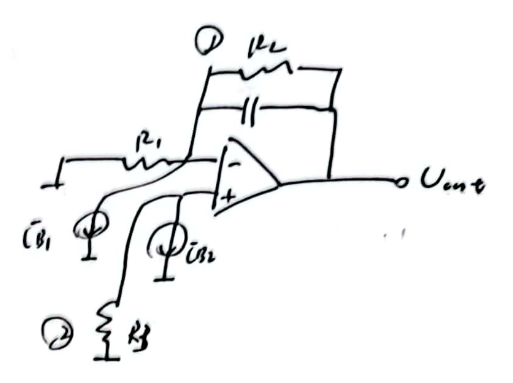
\includegraphics[scale=0.8]{16.jpg}
    \captionsetup{labelformat=empty}
    \caption{}
    \label{16}
\end{figure}

For one possible solution, we can add a resistor in parallel with the capacitor. The DC bias current flows through the resistor, and the AC signal flows through the capacitor. 

Or we can add resistor to the positive input. In this way, the inputs of op amp have the same bias. 

\subsection*{Speed Limitations}

For a single-ended input op amp: 

$$H(s)=\frac{A_o}{1+\frac{s}{w_0}}$$

Changed to two-end input: 

\begin{figure}[htbp]
    \centering
    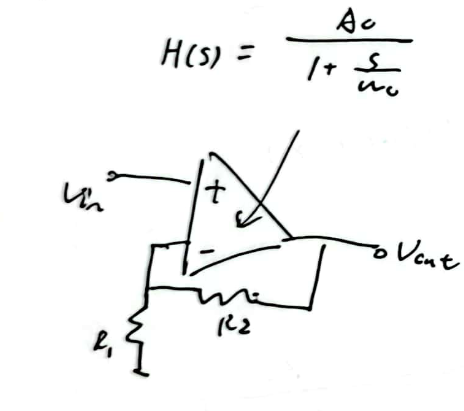
\includegraphics[scale=0.6]{18.jpg}
    \captionsetup{labelformat=empty}
    \caption{}
    \label{18}
\end{figure}

$$\frac{V_{out}}{V_{in}}(s)=\frac{\frac{A_o}{1+\frac{s}{w_0}}}{\frac{A_o}{1+\frac{s}{w_0}}\frac{R_1}{R_1+R_2}+1}=\frac{A_o}{\frac{s}{w_0}+1+A_o\frac{R_1}{R_1+R_2}}$$

\begin{figure}[htbp]
    \centering
    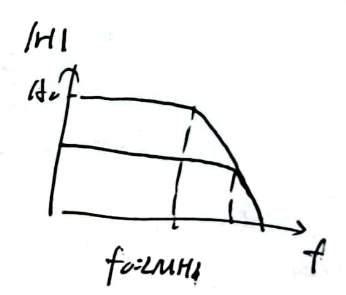
\includegraphics[scale=0.6]{17.jpg}
    \captionsetup{labelformat=empty}
    \caption{}
    \label{17}
\end{figure}

It can be seen that the gain of the two-terminal input is reduced compared with that of the single terminal, but the bandwidth is increased. 

\subsection*{Slew Rate}

\begin{figure}[htbp]
    \centering
    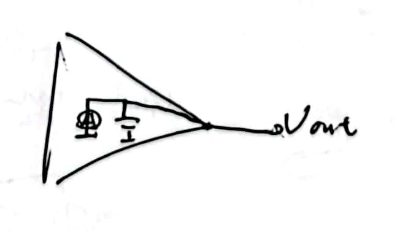
\includegraphics[scale=0.4]{20.jpg}
    \captionsetup{labelformat=empty}
    \caption{}
    \label{20}
\end{figure}

The op amp output can be regarded as a current source and a capacitor. As the input increases, the capacitor slowly charges and the output slowly increases. The charging speed of the capacitor is limited, so the output change rate of the op amp is limited, that is, the voltage swing rate. 

\begin{figure}[htbp]
    \centering
    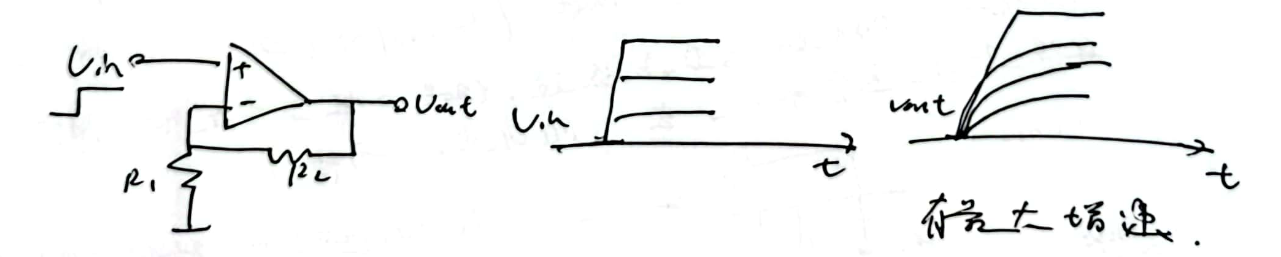
\includegraphics[scale=0.6]{19.jpg}
    \captionsetup{labelformat=empty}
    \caption{}
    \label{19}
\end{figure}

\section*{Link}

\href{https://www.bilibili.com/video/BV1FD4y1R7Ah?p=44&vd_source=1d0c07486a3bd3b0adb8ac548bf6453e}{Razavi Electronics Circuits 1: lectrue 44}

\href{https://www.bilibili.com/video/BV1FD4y1R7Ah?p=45&vd_source=1d0c07486a3bd3b0adb8ac548bf6453e}{Razavi Electronics Circuits 1: lectrue 45}
\end{document}